
\section*{Problema P10.22}

\renewcommand*\thesection{10.22}
\numberwithin{equation}{section}

\begin{center}
    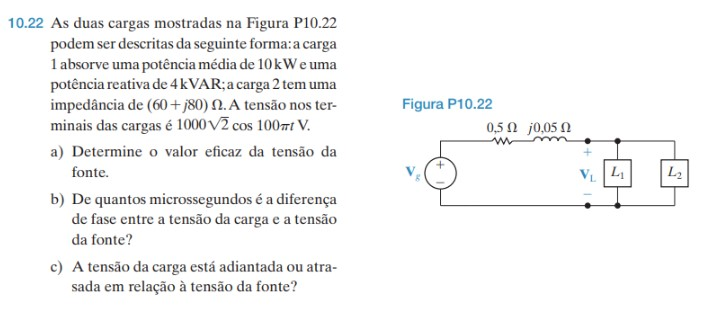
\includegraphics[scale=1.0]{P10.22.jpg}
\end{center}

\subsection*{(a)}

Temos as seguintes informações dadas:

\[ S_1 = 10000 + j4000 \;\textrm{VA} \quad , \quad Z_2 = 60 + j80 \;\Omega \quad , \quad V_1 = V_2 = 1000\phase{0^{\circ}} \;\textrm{V} \]

Em $L_1$, temos    

\[ S_1 = V_1 \cdot (I_1)^* \quad \Rightarrow \quad I_1 = \left(\frac{S_1}{V_1}\right)^* \quad \Rightarrow \quad I_1 = 10 -j4 \;\textrm{A}\]

Uma vez calculado $I_1$, agora calculamos a impedância da carga $L_1$.

\[ Z_1 = \frac{V_1}{I_1} = \frac{1000}{10 - j4} = 86,2 + j34,5 \;\Omega \]

Agora vamos calcular a corrente $I_2$ da carga $L_2$.

\[ I_2 = \frac{V_2}{Z_2} = \frac{1000}{60 + j80} = 6 - j8 \;\textrm{A}  \]

% Assim, a potência na carga $L_2$ é

% \[ S_2 = V_2 \cdot (I_2)^* = (1000)(6 - j8)^* = 6000 + j8000  \]

Assim, a corrente fornecida pela fonte é

\[ I_g = I_1 + I_2 = 10 -j4 +  6 - j8 \;\textrm{A} = 16 - j12 \;\textrm{A} \]

A impedância $Z_{in}$ vista pela fonte é

\[ Z_{in} = 0,5 + j0.05 + (Z_1 \; // \; Z_2) \]

\[ Z_{in} = 0,5 + j0.05 + \frac{1}{\frac{1}{86,2 + j34,5} + \frac{1}{60 + j80}} \]

\[ Z_{in} = 0,5 + j0.05 + 40 + j30 = 40,5 + j30,05 \;\Omega \]

Finalmente, a tensão da fonte é

\[ V_g = Z_{in} \cdot I_g = (40,5 + j30,05)(16 - j12) = 1008,6 - j5,2 \;\textrm{V}\]

\[ \boxed{V_g = 1008,6 \phase{-0,295^{\circ}}  \;\textrm{V}} \]

\subsection*{(b)}

Usando proporcionalidade (regra de três simples), temos   

\[ \frac{T}{\Delta t} = \frac{360^{\circ}}{\Delta \phi}  \]

onde $\Delta \phi$ é a diferença de fase entre os sinais. Portanto, usando $T = \frac{2\pi}{\omega}$,

\[ \Delta t = \frac{2\pi}{\omega} \frac{\Delta \phi}{360^{\circ}} \]

Substituindo,

\[ \Delta t = \frac{2\pi}{100\pi} \frac{0,295^{\circ}}{360^{\circ}} \]

\[ \boxed{\Delta t = 16,39 \;\mu\textrm{s}} \]

\subsection*{(c)}

$V_L$ está $\Delta \phi = 0,295^{\circ}$ adiantada em relação a $V_g$.









